\documentclass[10pt, a4paper]{article}
\usepackage[utf8]{inputenc}
\usepackage[paper=a4paper, left=4.0cm, right=4.0cm, bottom=1.5cm, top=3.5cm]{geometry}
\usepackage{mathtools}
\usepackage{float}
%\usepackage{graphicx}
\usepackage[]{algorithm2e}
\usepackage{amssymb}
\usepackage{subcaption}

\usepackage[conEntregas]{caratula}

\begin{document}

\titulo{Trabajo Pr\'actico 1}

\fecha{10/04/2015}

\materia{Introducción al Procesamiento Digital de Imágenes}

\integrante{Dellanzo, Claudia Antonella}{019/13}{antodellanzo@gmail.com}
\integrante{Julián Bayardo}{850/13}{julian@bayardo.info}
% Pongan cuantos integrantes quieran

\maketitle
\tableofcontents

\newpage

\section{Introducción}

El objetivo de este trabajo prático es implementar un algoritmo para realzar imágenes a través de la ecualización de histogramas siguiendo lo propuesto en el paper \textit{Adaptive extended piecewise histogram equalisation for dark image enhancement} \cite{paper}. Aparte de esto, se buscará realizar un estudio sobre la selección de parámetros (en cuántos histogramas partir el original y la selección de $\alpha$ y  $\beta$).

\section{Implementación}

Para la implementación del algoritmo seguimos el propuesto en el paper, el cual es:

\begin{figure}[H]
	\centering
    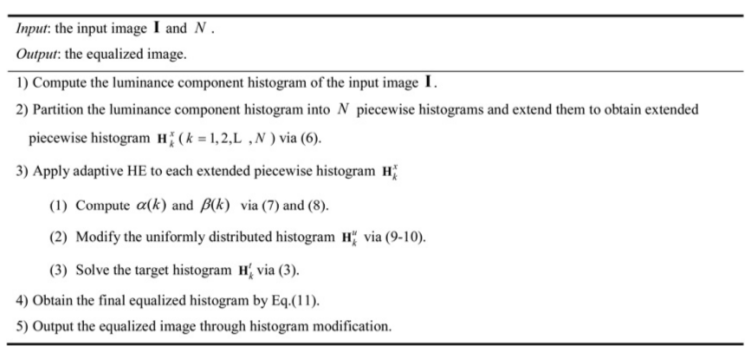
\includegraphics[width=\textwidth]{algoPaper.png}
    \caption{Algoritmo propuesto}
\end{figure}

El método llamado \textbf{AEPHE} toma como parámetro obligatorio de entrada la imagen y le aplica todas las transformaciones propuestas. Aparte, hay otros parámetros de entrada opcionales:
\begin{itemize}
\item \textit{Alphas:} Toma un vector de $\alpha$'s, los cuales serán aplicados en orden a cada subhistograma generado durante el algoritmo.
\item \textit{Betas:}  Toma un vector de $\beta$'s, los cuales serán aplicados en orden a cada subhistograma generado durante el algoritmo.
\item \textit{Gammas:} Toma un vector de $\gamma$'s, los cuales serán aplicados en orden a cada subhistograma generado durante el algoritmo.
\item \textit{number\textunderscore of\textunderscore histogramas:} Cantidad de histogramas en los que se desea partir el histograma original de la imagen de entrada. El valor es $3$ por defecto.
\item \textit{discretization\textunderscore bin\textunderscore width:} Cantidad de \textit{bins} en los que se dividirá el histograma al momento de realizar la conversión para trabajar con enteros o floats. El valor es $1/255$ (255 bins) por defecto. 
\item \textit{plot\textunderscore intermediate\textunderscore histograms:} Booleano que indica si se quiere ir mostrando las figuras de todos los subhitogramas generados durante la ejecución del algoritmo. El valor es \textit{False} por defecto.
\end{itemize}

La razón por la cual tomamos vectores de valores en algunos parámetros será explicada posteriormente cuando hablemos sobre la experimentación y los problemas con los que nos encontramos al realizar los mismos.

Si el vector de $\gamma$'s no se especifica, tomamos todos los valores como 0 ya que dicho parámetro no contribuye notablemente al realce de la imagen. Si alguno de los otro dos vectores (vector de $\alpha$'s o $\beta$'s) es nulo, luego se procede a calcularlos de la manera que lo indica el paper:

\begin{equation}
\alpha = \dfrac{M_{i}}{M_{i} + M_{c}}
\end{equation}
\begin{equation}
\beta = \dfrac{M_{c}}{M_{i} + M_{c}}
\end{equation}

\begin{figure}[H]
	\centering
    \begin{subfigure}{0.5\textwidth}
        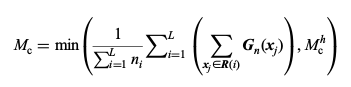
\includegraphics[width=0.9\textwidth]{calculo-Mc.png}
    \end{subfigure}\hfill
    \begin{subfigure}{0.5\textwidth}
        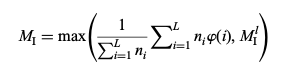
\includegraphics[width=0.9\textwidth]{calculo_Mi.png}
    \end{subfigure}\hfill
\end{figure}

\section{Experimentación}


\newpage 

\begin{thebibliography}{9}
\bibitem{paper}
Zhigang Ling, Yan Liang, Yaonan Wang, He Shen, Xiao Lu. \textit{Adaptive extended piecewise histogram equalisation for dark image enhancement.} IET Image Processing. 2015.
\end{thebibliography}


\end{document}